\section{Antenner för VHF/UHF/SHF}

\subsection{Allmänt}

Alla antenner fungerar efter samma principer. Principerna för
kortvågsantenner kan därför tillämpas även för antenner för högre
frekvenser. Byggmåtten på en VHF/UHF-antenn är betydligt mindre än för
en motsvarande KV-antenn. Jämför \(\lambda\) = ca 2~m vid 145~MHz och
\(\lambda\) = ca 80~m vid 3,5~MHz. Det är därför möjligt att bygga
riktantenner med rimliga dimensioner för VHF/UHF, även om flera
element används.

Om man bortser från rundstrålande vertikalantenner för trafik på korta
avstånd och mobil trafik, så används riktantenner främst p.g.a. den
större räckvidden. En riktantenns egenskaper uttrycks i första hand i
storheterna strålningsvinkel, antennvinst, fram/backförhållande och
halvvärdesbredd.

Eftersom polarisationsvridning sällan förekommer vid högre frekvenser,
är det viktigt att sändar- och mottagarantenner har samma
polarisationsriktning. Horisontell polarisation anses vara bättre
lämpad för långa distanser, eftersom vågor med horisontell
polarisation böjer av bättre över horisontella formationer (bergryggar
etc). Även passage genom skogspartier går bättre med horisontellt
polariserade vågor. Antenner med horisontell polarisation används
därför ofta för SSB- och CW-trafik på långa avstånd och utmed
markytan. Sådan trafik sker i allmänhet från fasta stationer.

För mobil trafik och lokal fast trafik används dock antenner med
vertikal polarisation. Vertikala antenner ger de önskvärda
rundstrålande egenskaperna för mobil trafik och är bäst lämpade att
montera på fordon.

\subsection{Riktantenner}

En \(\lambda/2\)-antenn strålar vinkelrätt ut från antennledaren och
runt omkring den.  Placeras ett reflektorelement (längd
\(\approx\lambda/2 + 5\%\)) bakom antennen på ett avstånd av \(\approx
\lambda/5\) så reflekteras den bakåtriktade strålningen delvis
framåt. En större del av energin kommer då att samlas i en
riktning. Med ett direktorelement (längd \(\approx\lambda/2 - 5\%\))
framför det strålande elementet på ett avstånd av
\(\approx\lambda/10\) så kommer utstrålningsvinkeln att bli mindre.

\subsection{yagiantenner}

\begin{figure}
  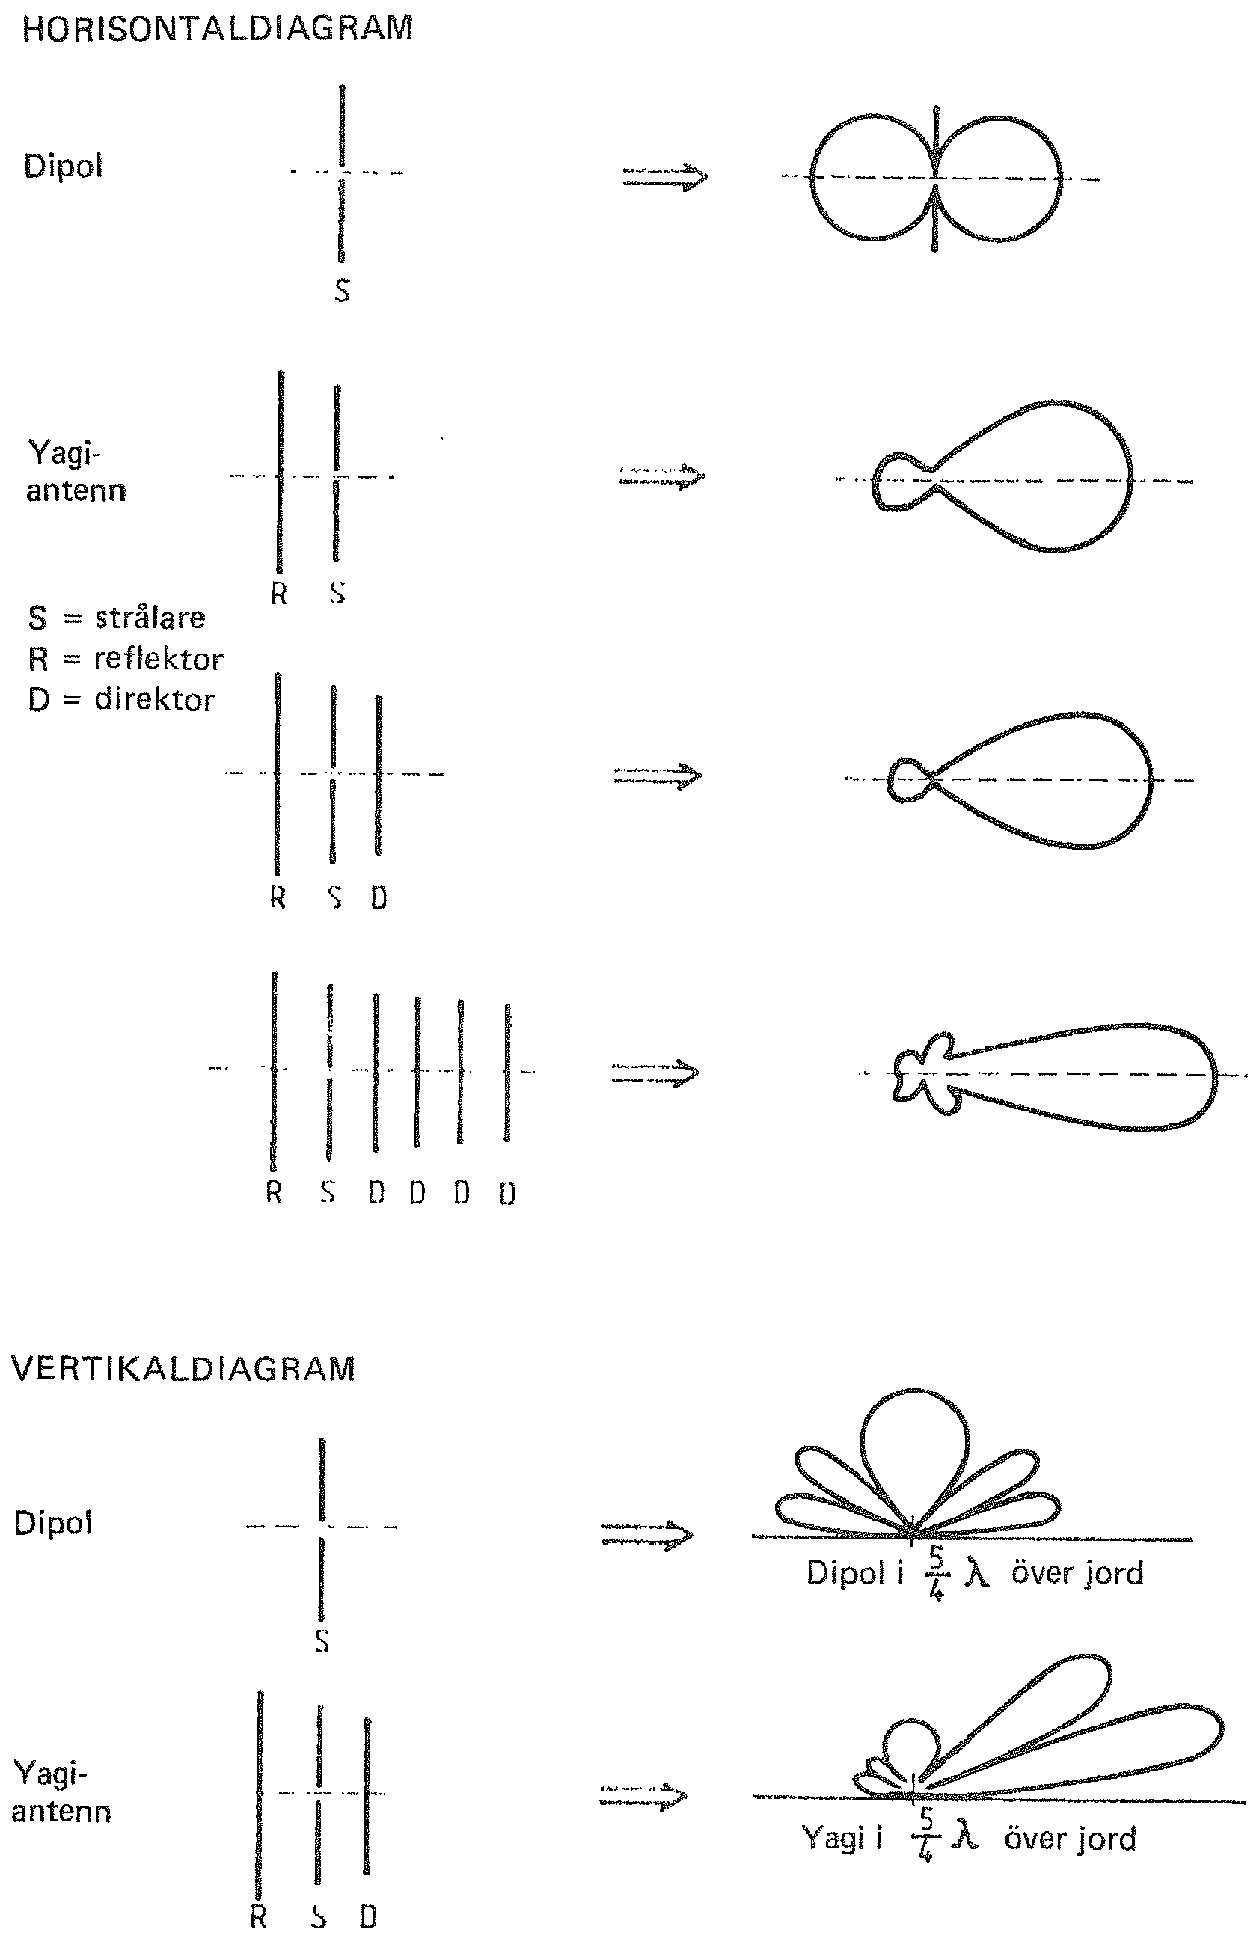
\includegraphics[width=\textwidth]{images/bild_2_6-20.png}
  \caption{Strålningsdiagram för horisontell yagiantenn}
  \label{fig:bildII6-20}
\end{figure}

Bild \ref{fig:bildII6-20}

Den typ av riktantenn, som består av en strålare, en passiv reflektor
samt ett antal passiva direktorer, kallas yagiantenn.

Yagiantennen kan utföras med olika antal direktorelement i
kombination med olika längd.

Det finns tre sätt att optimera en riktantenn, nämligen maximal
riktverkan, minimum sidlober och maximalt fram/backförhållande. Dessa
egenskaper är, emellertid ej möjliga att uppnå samtidigt. Ökas t.ex.
antalet element, så ökar den s.k. antennvinsten genom att
öppningsvinkeln på strålningen blir mindre, men samtidigt minskar
matningsimpedansen och den användbara bandbredden.

\hilight{TODO: antennvinsten bestäms väl snarare av längden på bommen, eller?}

\subsection{Gruppantenner}

Ordnas flera riktantenner vid sidan av och/eller över varandra så
erhålls en s.k. gruppantenn. Ett sådant arrangemang av s.k. stackade
antenner ger en ännu mindre öppningsvinkel på strålningen vertikalt
och/eller horisontellt. Därigenom erhålls ytterligare antennvinst.

\subsection{Parabolantenner}
\textbf{
HAREC a.\ref{HAREC.a.6.1.6}\label{myHAREC.a.6.1.6}
}

Särskilt på frekvenser i mikrovågsområdet och högre har radiovågorna i
stort sett samma utbredningsegenskaper som ljusets.  Behöver stor
riktverkan uppnås på dessa höga frekvenser, används ofta en parabolisk
yta som spegel bakom själva antennen.  Jämför med reflektorn i en
ficklampa.

Den egentliga antennen (den s.k. mataren), vars strålning är riktad
mot parabolen för att reflekteras, kan vara utformad på många
sätt. Eftersom parabolens storlek står i omvänd proportion till
frekvensen, så används av praktiska skäl inte paraboliska reflektorer
på låga frekvenser.

\subsection{Övriga antenntyper}

Rundstrålande antenner: Ground plane, \(\lambda/4\)-, \(\lambda/2\)-,
\(5\lambda/8\)-antenner m.fl.

Riktantenner: Quad-, HB9CV-, helical-, parabol- och hornantenner m.fl.
